\documentclass[12pt]{article}
\usepackage{amsthm}
\usepackage{libertine}
\usepackage[utf8]{inputenc}
\usepackage[margin=.6in, includefoot]{geometry}
\usepackage{amsmath,amssymb}
\usepackage{multicol}
\usepackage[shortlabels]{enumitem}
\usepackage{siunitx}
\usepackage{cancel}
\usepackage{graphicx}
% \usepackage{pgfplots}
\usepackage{listings}
\usepackage{tikz}
\usepackage{csquotes}
\usepackage{xcolor-solarized}
\usepackage[colorlinks, allcolors=solarized-blue]{hyperref}
% custom
\usepackage{shortcuts}
\usepackage{fancyhdr}
\pagestyle{fancy}
\fancyhf{}
\usepackage{lastpage}
\usepackage{setspace}
\usepackage{thmtools}
\usepackage{cleveref}
\usepackage{physics}
\usepackage{caption}
\usepackage{subcaption}
\usepackage[backend=biber, style=numeric]{biblatex}

\addbibresource{./bib.bib}

\newtheorem{definition}{Definition}
\newtheorem{remark}{Remark}

\MakeOuterQuote{"}
% \pgfplotsset{width=10cm,compat=1.9}
% \usepgfplotslibrary{external}

% \fancyfoot[C]{{\small\thepage \hspace{0.05cm} / \hspace{0.05cm}\textcolor{gray}{\pageref*{LastPage}}}}
% header rule
% leave any blank to not include it
\newcommand{\titlename}{Dynamical Systems and Climate Modeling}
\newcommand{\subtitlename}{MATH376 - Nonlinear Dynamics Final Project}



\begin{document}
\pagestyle{plain}
\thispagestyle{empty}

\noindent
{\huge\textbf{\titlename}}\\\\
{\large \subtitlename}\\\\
\rule[2ex]{\textwidth}{2.5pt}
% TODO: picture here?
\begin{center}
{\small Louis Meunier}\\
{\small louis.meunier@mail.mcgill.ca}\\
{\small 261097560}
\end{center}
% ---
\setstretch{1.4}
\begin{figure*}[!ht]
    \centering
    \includegraphics*{figures/temp.png}
\end{figure*}
\begin{abstract}
    The atmosphere is a notoriously complicated system to effectively model. From a mathematical standpoint, there is a necessity for a particular amount of simplicity and physical assumptions in order for models to be reasonable to analyze. On the other hand, excessive simplifications lead to misrepresentative results which, while mathematically convenient, are, from an application standpoint, functionally useless.

    In this article, we will give an overview of approaches that attempt to thread the line of these differing necessities, with a focus on Delay Differential Equations (DDEs), their effectiveness in modeling natural phenomena, and some methods used to analyze them.
\end{abstract}

\small{\tableofcontents}

\section{Introduction}

Climate modeling tools and strategies have changed significantly in recent history. In short, what began as a largely computational endeavor has begun to be approached in recent years as a more rigorous physical and mathematical endeavor.

For one, \emph{General Circulation Models} (GCM's), are the prototypical example of large-scale models of the earth designed with a focus on addressing physical complexity as approximately as possible. These models rely heavily on computation and accounting for huge sets of variables and parameters. While these models are still in wide use today, particularly for the sake of long-term climate modeling, they suffer much criticism for their inate complexity, high uncertainties, and the suspect practice of parameter tuning \cite{gcmobsolete} \cite{climatedde}.

% TODO: add ideas about feedback looops and their relation to ddes/odes

\section{About DDE's: Background}

For ease of discussing specific DDE models in the context of climate phenomena in the following sections, the next section will review some elementary theory of DDEs.

\begin{definition}[DDE]
    A Delay Differential Equation, or DDE, is a differential equation of the general form \begin{equation}\label{eqn:dde}
    \dot{x}(t) = f(x(t), x_t, t),
    \end{equation}
    where $x_t = \{x(\tau) : \tau \leq t\},$ with $\tau$ being an arbitrary time. In this way, the $x_t$ term represents the reliance of $\dot{x}$ on past conditions\cite{DDEtext} \cite{functionalDDEtext}.

    The majority of the models to follow will adopt a discrete delay term $x_t$. In this way, we may rewrite \cref{eqn:dde} as \begin{equation}\label{eqn:discretedde}
        \dot{x}(t) = f(x(t), x(t + \tau_1), x(t+\tau_2), \cdots, t).
    \end{equation}
\end{definition}


\begin{remark}
    In the case that $x_t = 0 \forall t$, then \cref{eqn:dde} becomes the standard form of an ordinary differential equation.
\end{remark}

\subsection{Method of Steps}

The \emph{method of steps} is a typical stepwise method used to compute solutions of delay differential equations. It is also implemented in many softwares, in more optimized forms \cite{DDEtext}\cite{functionalDDEtext}\cite{ndsolvedde}. To illustrate, consider the simple DDE, with constant delay,
\begin{equation}\label{eqn:ddesimpleoriginal}
    \dot{x}(t) = f(x(t), x(t-\tau))
\end{equation}
defined on $t \geq 0$. Typically, we are given some initial condition for the system, in the form of a function defined over "past time" of the system; say, $\theta_0 : [- \tau, 0] \to \mathbb{R}^n$. 

We can then solve for the solution $\theta_1(t)$ to $\dot{x}(t)$ over the time interval $[0, \tau]$, by plugging $\theta_0$ into \cref{eqn:ddesimpleoriginal}:\begin{equation}
    \dot{\theta_1}(t) = f(\theta_1(t), \theta_0 (t - \tau)).
\end{equation}
This gives an initial value problem, where $\theta_1(0) = \theta_0(0)$; more generally, we have that $\theta_n((n-1)\tau) = \theta_{n-1}((n-1)\tau)$, which intuitively ensures "smooth" transitions between iterations. Continuing in this way, we can find the solution to \cref{eqn:ddesimpleoriginal} over an arbitrary time range $[(n-1)\tau, n\tau],$ where $n \in \mathbb{N}$, as 
 \begin{equation}
    \dot{\theta_n}(t) = f(\theta_{n}(t), \theta_{n-1}(t-\tau)), \quad \theta_n((n-1)\tau) = \theta_{n-1}((n-1)\tau).
\end{equation}

Note that there was nothing special about specifying that we are moving forward in time to find solutions; this is simply the most natural manner of interpreting these equations. We could work backwards in time over $[-(n-1)\tau, -n \tau], n \in \mathbb{N}$ to find solutions then as well.

Overall, then, this method yields a piecewise solution (or, aptly, "indexed" solutions):
\begin{equation}
    x(t) = \begin{cases}
        \theta_0(t) & t \in [- \tau, 0]\\
        \theta_1(t) & t \in [0, \tau]\\
        \vdots & \vdots \\
        \theta_n(t) & t \in [(n-1)\tau, n\tau]\\
        \vdots & \vdots
    \end{cases} \equiv \theta_{\tilde{n}}(t), \quad \text{ where } \tilde{n} :=  \lceil\frac{t}{\tau}\rceil.
\end{equation}

\subsection{Example 1 - $\dot{x}(t) = kx(t - \tau)$}

To demonstrate the method of steps more concretely, consider the following DDE with constant delay: \begin{equation}
    \dot{x}(t) = kx(t- \tau),
\end{equation}
where $k \neq 0$ an arbitrary parameter, and we are given that $\theta_0(t):[-\tau, 0] = 1$. Solving the first few iterations of this simple model, we have:
\begin{alignat}{2}
    \dot{x(t)} = kx(t-\tau) && \\
    \dot{\theta_1}(t) = k \theta_0(t-\tau), \quad \theta_1(0) = \theta_0(0) = 1 && \quad t \in [0, \tau]\\
    \implies \dot{\theta_1} = k \implies \theta_1(t) = kt + \theta_1(0) \implies \theta_1(t)= kt + 1\\
    \dot{\theta_2}(t) = k \theta_1(t - \tau), \quad \theta_2(\tau) =\theta_1(\tau) = k \tau + 1 && \quad t \in [\tau, 2\tau]\\
    \implies \theta_2 = \theta_2(\tau) + \int_{\tau}^{t} \theta_1(t' - \tau) \dd{t'}\\
    \implies \theta_2(t) = k\tau + 1 +k(t - \tau)(\frac{1}{2}k(t - \tau) + 1)\\
    \dots
\end{alignat}

An example solution of this equation, with $k = -1.7, \tau = 0.6,$ and initial condition $\theta_0:[-0.6, 0] \to \mathbb{R}, t \mapsto 1$, is shown in \cref{fig:simpleddeimage}.

\begin{figure}[!ht]
    \centering
    \begin{subfigure}{.5\textwidth}
      \centering
      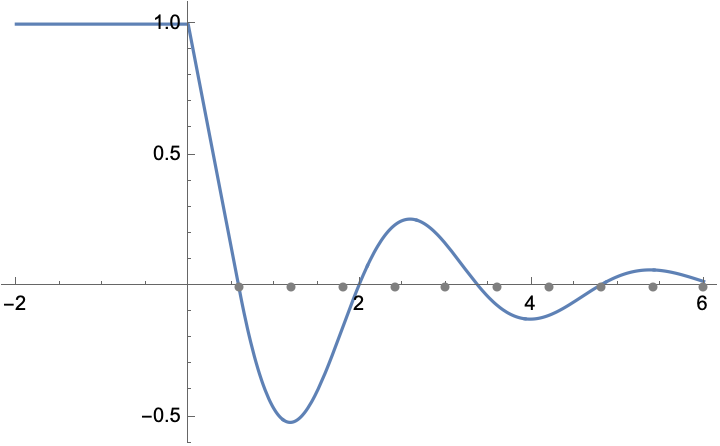
\includegraphics[width=.9\linewidth]{figures/simpledde.png}
      \caption{Solution to $\dot{x}(t) = -1.7x(t - 0.6)$}
      \label{fig:simpleddeimage}
    \end{subfigure}%
    \begin{subfigure}{.3\textwidth}
    %   \centering
      \begin{lstlisting}[basicstyle=\footnotesize]
        \\[Tau] := 0.6
        k := -1.7
        sol := NDSolve[
            {
                x'[t] == k*x[t - \[Tau]], 
                x[t /; t <= 0] == 1
            }, x, 
            { t, -5, 10*\[Tau] }
        ]
        Plot[
            Evaluate[x[t] /. sol], 
            {t, -2, 10*\[Tau]}
        ]
      \end{lstlisting}
      \caption{Mathematica Code}
      \label{fig:sub2}
    \end{subfigure}
    \caption{Numerically computed solution to \cref{eqn:ddesimpleoriginal}, in Mathematica}
    \label{fig:mathematicamagicsimple}
\end{figure}

\begin{remark}
    In the particular case that $k = -1, \tau = \frac{\pi}{2}$, we have \[
    \dot{x}(t) = -x(t - \frac{\pi}{2}),
    \]
    that is, the derivative of $x(t)$ is the negative of itself, phase shifted $\frac{\pi}{2}$. By inspection, its rather clear that the solution is simply \[
    x(t) = \cos t.    
    \]
\end{remark}

\subsection{Example 2 -  $\dot{x}(t) = rx(t)(1 - \frac{x(t-\tau)}{K})$}

The standard, well-studied, logistic equation, formulated by Verhulst, is of the form \begin{equation}
    \dot{x}(t)= rx(t)\left(1 - \frac{x(t)}{K}\right),
\end{equation}

where $r, K$ are strictly positive parameters. 

Consider the modified, delayed form of this equation, formulated by Hutchinson \cite{Hutchinson}:
\begin{equation}\label{eqn:hutchinson}
    \dot{x}(t) = rx(t)\left(1 - \frac{x(t - \tau)}{K}\right).
\end{equation}

In the standard logistic equation, the "inner term" assumes that growth rate is relative to the current population, $x(t)$. Here, the inclusion of the delay term $\tau$ implies that the growth rate is relative to previous populations, indicating some type of "lag time" of effects \cite{ddesinglespecies}.

The method of steps could be used to find some solutions, but would be rather slow algebraically. As we are generally more interested with the dynamics of a system such as this rather than any potential analytic solution we could derive, we will, in this section, focus on more quantitative methods we may use to study DDEs, making sure to link these techniques back to the well-known theory of dynamics of ODEs.

\subsubsection{Steady States, Stability Analysis}

We can compute steady states of \cref{eqn:hutchinson} identically to "ordinary" dynamical systems:
\begin{align*}
    \dot{x}(t) = 0 &\iff rx(t)\left(1 - \frac{x(t - \tau)}{K}\right)\\
    &\iff x(t) = 0 \quad \vee \quad x(t - \tau) = K\\
    &\text{Let } x^*_1 \equiv 0, x^*_2 \equiv K
\end{align*}

Consider $x^*_1$. For small enough perturbations from the origin, $\dot{x} \approx rx(t)$ (neglecting the inner term; this is particularly "valid" if $K >> 0$). This has a simple exponential solution $x(t) = X_0 e^{rt}$, hence the origin is unstable as we have that $r >0$.

To analyze $x^*_2$, we first manipulate \cref{eqn:hutchinson}:
\begin{align*}
    \dot{x}(t) = rx(t)\left(1 - \frac{x(t - \tau)}{K}\right) &= \frac{r}{K}x(t)\left(K - x(t - \tau)\right)\\
    \tilde{x}(t) := x(t) - K \implies \dot{\tilde{x}}(t) &= \frac{r}{K}(\tilde{x}(t) + K)(-\tilde{x}(t - \tau))\\
    &= \underbrace{-\frac{r}{K}\tilde{x}(t)\tilde{x}(t - \tau)}_{\text{nonlinear}} \underbrace{- r \tilde{x}(t - \tau)}_{\text{linear}}
\end{align*}

Just as in ODE-based dynamical systems, we can perform linear stability analysis in a similar way even when delays are concerned. In this case, the LHS term involves both $\tilde{x}(t)$ and $\tilde{x}(t - \tau)$ and is thus nonlinear in $\tilde{x}$. Note that despite one of these terms not being "of the same time", this still results in a nonlinear term (this is particularly clear if $\tau = 0$). This gives a linearization \begin{equation}\label{eqn:linearization}
    \dot{\tilde{x}}(t) = -r \tilde{x}(t - \tau).
\end{equation}

This, again, looks like an exponential solution would fit, if the delay term were not present. To analyze this, we introduce the following extension of the characteristic polynomial to DDEs.

\subsubsection{Characteristic Equation, Bifurcation Analysis}

The \emph{characteristic equation} of a linear, homogenous \textit{ODE} of the form \[
0 = A_0y + A_1y' + \cdots + A_ny^{(n)}
\]
is a polynomial of the form \[
0 = A_0 + A_1r + \cdots + A_n r^n,
\]
whose roots $r_i$ allow us to find the general solution to $y$. This is derived from assuming a general complex exponential solution of the form $x(t) = x_0 e^{rt}$, which, when substituting into the original ODE, yield the characteristic equation.

Similarly, suppose we are working with a linear DDE of the form \[
\dot{x}(t) = A_0 x(t) + A_1x(t -\tau_1) + \cdots + A_n x(t - \tau_n).
\]
Assuming a solution of the form $x(t) = x_0e^{rt} \implies x(t - \tau_1) = x_0e^{r(t - \tau)}, \dots,$ then after substituting into the original DDE, we have \begin{align}
    re^{rt} = A_0e^{rt} + A_1e^{r(t - \tau_1)} + \cdots + A_n e^{r(t - \tau_n)},
\end{align}

which, after simplifications, gives the characteristic equation of linear DDEs:

\begin{equation}\label{eqn:characteristic}
    r = A_0 + A_1e^{-r\tau_1} + \cdots + A_ne^{-r\tau_n}.
\end{equation}
Note that $r \in \mathbb{C}$ by our assumptions, as previously.

We can then, as before, solve for the roots of this polynomial and find solutions. However, this is now a polynomial in terms of exponentials as well as a linear term, and thus presents far more challenges in solving analytically.

To see this, consider again \cref{eqn:linearization} from our example. In terms of our general formula \cref{eqn:characteristic}, we have $n = 1$, $A_0 = 0$ and $A_1 = -r$. Since we are already using $r$ as a parameter here, let $\lambda$ take the functional place of $r$ in the characteristic polynomial. Then, we have \begin{equation}\label{eqn:lambda}
    \lambda = -re^{-\lambda \tau}.
\end{equation}

One manner to solve this equation for $\lambda$ is via the following function.

\begin{definition}[Lambert $W$ Function]
    The Lambert $W$ function, $W(x)$, is defined (on the real line) as the solution to
    \begin{equation*}
    W(x)e^{W(x)} = x; \quad W : [- \frac{1}{e}, \infty] \to \mathbb{R}.
    \end{equation*}
    In the case that $x > 0$, the function yields a single real solution. If $x \in [-\frac{1}{e}, 0),$ $W$ yields two solutions; these are typically denoted $W_0(x)$ and $W_{-1}(x)$. The former remains $W_0(x) \geq -1 \forall x$, while $W_{-1}(x) \leq -1 \forall x \in [- \frac{1}{e}, 0)$\cite{wlamber}.
    \begin{figure*}[!ht]
        \centering
        \includegraphics*[width=0.4\textwidth]{figures/wlambert.png}
        \caption{Real parts of $W_0(x)$ and $W_{-1}(x)$ Lambert $W$ function.}
    \end{figure*}
    Moreover, the Lambert $W$ function has complex solutions (branches), denoted $W_k(x)$ for $k \in \mathbb{Z}$.
\end{definition}

Using numerical methods, we could use this function to find solutions to \cref{eqn:lambda} for $\lambda$ in terms of $r$ and $\tau$, and hence find the stability of the steady state as a function of the parameter and the time delay. Rather, for a more clear analytical solution, let $\lambda = \alpha + \beta i \in \mathbb{C} =\Re\lambda+ \Im\lambda i$. Substituting this into \cref{eqn:lambda}:
\begin{align*}
    \alpha + \beta i = -re^{-(\alpha + \beta i)\tau} &= -re^{-\alpha\tau}e^{-\beta\tau i}\\
    &= -re^{-\alpha \tau}\left[\cos\left(\beta \tau\right) - i \sin \left(\beta\tau \right)\right]\\
    &\implies \alpha +re^{-\alpha \tau} \cos (\beta \tau) = 0 \quad (i)\\
    &\implies \beta - re^{- \alpha \tau}\sin(\beta \tau) = 0\quad (ii)
\end{align*}

As in stability analysis of ODEs, linearized stability depends on the sign of the real part of $\lambda$; $\alpha$ positive indicates instability, while $\alpha$ negative indicates stability. Moreover, this means that the stability of the system will change when $\alpha = 0$, that is, when $\lambda$ is purely imaginary. Let $\beta_c, \tau_c$ be the values of the imaginary part of $\lambda$ and the delay at this critical value. This yields:
\begin{align*}
    &(i)\implies r \cos (\beta_c \tau_c) = 0\implies \beta_c\cdot \tau_c = \frac{\pi}{2} + 2\pi n, n \in \mathbb{N} \implies \tau_c = \frac{\pi}{2 \beta_c},\dots\\
    &(ii) \implies \beta_c = r \sin (\beta_c \tau_c) = \pm r \\
    &\hspace{12em}\implies \tau_c = \frac{\pi}{2 r} + \cdots \implies \beta_c = \pm r
\end{align*}

Moreover, when $\tau \in [0, \tau_c]$, $\alpha < 0$ (stable); if $\tau > \tau_c$, then $\alpha > 0$ (unstable). When $\tau = \tau_c$, note that $\beta$, the imaginary parts, are nonzero, which strongly implies the existence of a Hopf bifurcation at this point \cite{scientificcomputing}. Indeed, at this point, we have \[
\lambda = \alpha + \beta i = \pm r i,
\]
which gives a solution to \cref{eqn:linearization} of \begin{equation}
    \tilde{x}(t) = Ce^{t \lambda} = Ce^{\pm r i t} = C \cos (rt),
\end{equation}
where $C$ a constant determined by initial conditions. Recall that $\tilde{x} = x - K$, so we have, moreover, \begin{equation*}\label{eqn:solutionhopf}
    x(t) = C \cos (rt) + K.
\end{equation*}
Supposing an initial condition of $x(t \leq 0)$, then we would simply have \[
x(t) = (x(t \leq 0) - K) \cos (rt) + K.   
\]

This sinuisoidal solution supports our hasty bifurcation prediction, as we do indeed have periodic motion appearing from a steady state. Moreover, this periodic motion occurs between limit cycles occurring at $x(t \leq 0)$ and $x(t\leq 0) + 2K$, and hence centered about $x = x^*_2 K$. This bifurcation is clear in the example solutions shown in \cref{fig:example2sol}, in which we include solutions plotted both in Cartesian coordinates $(x, y) \cong (t, x(t))$ and polar coordinates $(\theta, r) \cong (t, x(t))$ to better visualize the periodic behavior.

\begin{figure*}[!ht]
    \centering
    \includegraphics*[width=\linewidth]{figures/example2.png}
    \vspace{1.5em}
    \caption{Solutions in (above) Cartesian and (below) polar to Hutchinson's Equation with initial value $x(t \leq 0) = 0.5, K = 1.2, r = 1.5$. From left to right, $\tau < \tau_c$ ($x_2^* = K$ stable), $\tau = \tau_c$ (Hopf bifurcation), and $\tau > \tau_c$ ($x_2^* = K$ unstable, period-2 limit cycle). }
    \label{fig:example2sol}
    \vspace{2em}
    \includegraphics*[width=\linewidth]{figures/example2polar.png}
\end{figure*}

We can also summarize this stability analysis in a bifurcation diagram, \cref{fig:bifurcationdiagramex2}, noting that, in this case, we keep the parameters $r, K$ constant, and we plot $x$ as a function of the time delay $\tau$.

\begin{figure*}[!ht]
    \centering
    \includegraphics*[width=0.5\linewidth]{figures/bifurcationdiagramexample2.png}
    \caption{Bifurcation diagram of Hutchinson's equation; $r = 1.5, K = 1.2$.}
    \label{fig:bifurcationdiagramex2}
\end{figure*}

Having thoroughly examined \cref{eqn:hutchinson}, we proceed to use the methods established as we turn our focus to climactic models.
\newpage

\section{ENSO Modelling}

Typically, trade winds in the Pacific, blowing west, bring warm water from South America towards Asia, which is then replaced by deep cold-water upwelling. \emph{El Niño} and \emph{La Niña}, collectively referred to as the \emph{El Niño-Southern Oscillation} (ENSO), are two well-studied climate phenomena which break this trend \cite{aboutelnino}. Despite efforts, a wholly comprehensive understanding of ENSO has yet to be fully achieved.

In general, from observational data, it is clear that ENSO is a periodically occurring event, though which varying periodicity and strength in effect. Moreover, it is clear that both atmospheric and oceanic conditions couple to, in some manner, alter ENSO \cite{climatedde}. In particular, it has been noticed that sea-surface temperature (SST) fluctuations are directly related to wave patterns in the Pacific. In this way, the application of a DDE model is very appropriate; some form of delay exists with regards to how a particular quantity is effected.

In the following sections, we will discuss several ENSO DDE models, their mathematical relevance to physical patterns, and briefly analyze their behavior.

\subsection{Suarez ENSO Model}

One of the first DDE models for the ENSO effect was introduced by Suarez and Schopf in 1987 \cite{ensomodel}. The model is given as follows (modifying notation from the original text to more modern practices):
\begin{equation}\label{eqn:daoensomodel}
    \dot{h}(t) = h(t) - \left(h(t)\right)^3 - \alpha\cdot  h(t - \tau),
\end{equation}
in which $h$ represents anomaly of the \emph{thermocline depth}, $\alpha$ is a parameter value representing the scale of the delay term, and $\tau$ is the time delay (more specifically, $\tau$ in this model represents the wave transit time). The \emph{thermocline} refers to a layer of a body of water that divides the upper, surface layer (dubbed the "epipelagic zone") and the lower, cooler layer beneath \cite{thermocline}. The epipelagic zone, being the upper layer, is where atmospheric conditions most directly influence oceanic conditions. In this way, the depth and strength of the thermocline is often studied as a direct proxy for SST \cite{randomnino}\cite{climatedde}.

% TODO: add scientific reasoning - diagram of basin
\begin{remark}
    All plots, diagrams, and code listings, unless otherwise cited, are of my own creation. Source code, written in Mathematica, is posted \hyperref[here]{https://github.com/louismeunier/math376-final}
\end{remark}
\printbibliography
\end{document}
